\todo[inline]{unify lables of figures and tables}

\bigskip

\todo[inline]{\url{https://arxiv.org/pdf/cs/0108016.pdf}}
\todo[inline]{\url{https://www.cl.cam.ac.uk/~pes20/weakmemory/cacm.pdf}}
\todo[inline]{\url{https://mirrors.edge.kernel.org/pub/linux/kernel/people/paulmck/perfbook/perfbook-e2-rc9.pdf}}
% CBMC
\todo[inline]{\url{http://www.kroening.com/papers/tcad-sw-2008.pdf}}
\todo[inline]{\url{http://www.kroening.com/papers/tacas2004.pdf}}
\todo[inline]{\url{https://link.springer.com/content/pdf/10.1007/978-3-642-39799-8\_9.pdf}}

\newpage

\section{Introduction}

%% sequential consistency:
%% \emph{``the result of any execution is the same as if the operations of all the processors were executed in some sequential order, and the operations of each individual processor appear in this sequence in the order specified by its program''}.

% \todo[inline]{need for software verification}\noindent

Correctness of computer systems is critical in today's information age and although software verification made considerable progress in the last decade, it is still an ongoing research topic.
Testing alone however is not sufficient to validate parallel programs
communicating via shared memory on modern multiprocessor hardware,
% running on current multiprocessor hardware
% and communicating via shared memory,
% running on modern shared memory multiprocessor hardware
as fatal race conditions can have extremely low probabilities of occurrence.
The situation becomes even worse due to counter-intuitive behaviour introduced by certain hardware optimizations.
Without further knowledge about the underlying architecture, inexperienced developers of
concurrent
low-level
systems code like lock-free data structures, operating system kernels, synchronisation
% libraries,
primitives,
% compilers and so on might assume that the order of access to memory is \emph{sequentially consistent}
% compilers and so on might assume a total order of access to memory for any possible interleaving, where each process is executed in program order.
compilers,
% etc.\
and so on
might assume
% that
% \emph{``the result of any execution is the same as if the operations of all the processors were executed in some sequential order for every possible interleaving and the operations of each individual processor appear in this sequence in the order specified by its program''}
% the result of any execution is the same as if the operations of all processors were executed in some sequential order and the operations of each individual processor appear program order.
\emph{sequential consistency} \cite{ref:Lamport79}.
Unfortunately, none of the major hardware architectures follows this rather restrictive memory ordering model and allow
% memory access operations to be reordered
reordering of memory access operations
in various ways.
This opens the door for hard to find bugs caused by unexpected
% reorderings
behaviour
and
% needs to be prevented by
% requires careful use of the target architecture's memory barrier operations to ensure consistency.
requires a deep understanding of the target architecture's memory ordering model,
% as well as
accompanied by careful use of memory barrier operations to ensure consistency.
% referred to as \emph{sequential consistency} \cite{ref:Lamport79}.

% \bigskip

% For example, modern processors are equipped with a store buffer to speed up writes.

% \todo[inline]{counter-intuitive behaviour introduced by hardware optimizations}
% \todo[inline]{memory models}

% \bigskip

\tabulinesep=6pt
\noindent
\begin{table}[!hbt]
  \centering
  \begin{tabu}{|l|c|c|c|c|c|c|c|c|}
    \tabucline{2-}
    \multicolumn{1}{c|}{}
    & \rotatebox{90}{Alpha}
    & \rotatebox{90}{ARM}
    & \rotatebox{90}{Itanium}
    & \rotatebox{90}{MIPS}
    & \rotatebox{90}{POWER}
    & \rotatebox{90}{SPARC-TSO}
    & \rotatebox{90}{x86}
    & \rotatebox{90}{zSystems} \\
    \tabucline{2-}
    \firsthline
    Loads Reordered after Loads/Stores? & \cmark & \cmark & \cmark  & \cmark & \cmark & & & \\
    \hline
    Stores Reordered after Stores? & \cmark & \cmark & \cmark & \cmark & \cmark & & & \\
    \hline
    Stores Reordered after Loads? & \cmark & \cmark & \cmark & \cmark & \cmark & \cmark & \cmark & \cmark \\
    \hline
    Atomic Reordered with Loads/Stores? & \cmark & \cmark & & \cmark & \cmark & & & \\
    % \hline
    % Dependent Loads Reordered? & \cmark & & & & & & & \\
    % \hline
    % Dependent Stores Reordered & & & & & & & & \\
    \lasthline
  \end{tabu}
  % \caption{Summary of Memory Ordering}
  \caption{Memory Ordering on Different Architectures}
  \label{tbl:ordering}
\end{table}

% \subsection{Problem/Motivation}

% \todo[inline]{problems arising due to the unawareness of the specific architectures memory model}
% \todo[inline]{example for counter intuitive behaviour} \noindent

% Table \ref{tbl:ordering} shows that even the most restrictive architectures like the widely used x86

% The Intel-64 and AMD memory ordering models allow a load to be reordered with an earlier store to a different location, thus breaking sequential consistency.
% However, loads are not reordered with stores to the same location.
% Even though this is the only reordering allowed, it is sufficient for introducing counter intuitive behaviour, illustrated by the example given in Listing \ref{fig:intro:code}.

Table \ref{tbl:ordering} shows a rough overview of the memory ordering models used by different architectures.
Even the most restrictive -- like the x86 processors in our desktop computers -- allow loads to be reordered with an earlier store to a different location, thus breaking sequential consistency.
The reason for this particular reordering is a widely used optimization technique commonly referred to as \emph{store buffer}.

While caches improve subsequent repeated loads of a specific variable (after an initial cache miss),
\todo[noline]{stolen from perfbook}
it is also necessary to accommodate frequent concurrent stores from multiple processors to a set of shared variables.
In cache-coherent systems, if the caches hold multiple copies of a given variable, all the copies of that variable must have the same value.
Each store will therefore invalidate all copies of the old value, resulting in even more cache misses slowing down the computation. % significantly.
To remedy this situation, modern processors come equipped with store buffers, as shown in Figure \ref{fig:intro:store-buffer}.

% \todo[inline]{reordering introduced by store buffers}

\begin{figure}[!h]
  \centering
  % styles
\tikzstyle{box} = [draw, text centered, rounded corners]
\tikzstyle{processor} = [box, fill=blue!10]
\tikzstyle{buffer} = [box, fill=red!10]
\tikzstyle{cache} = [box, fill=green!10]

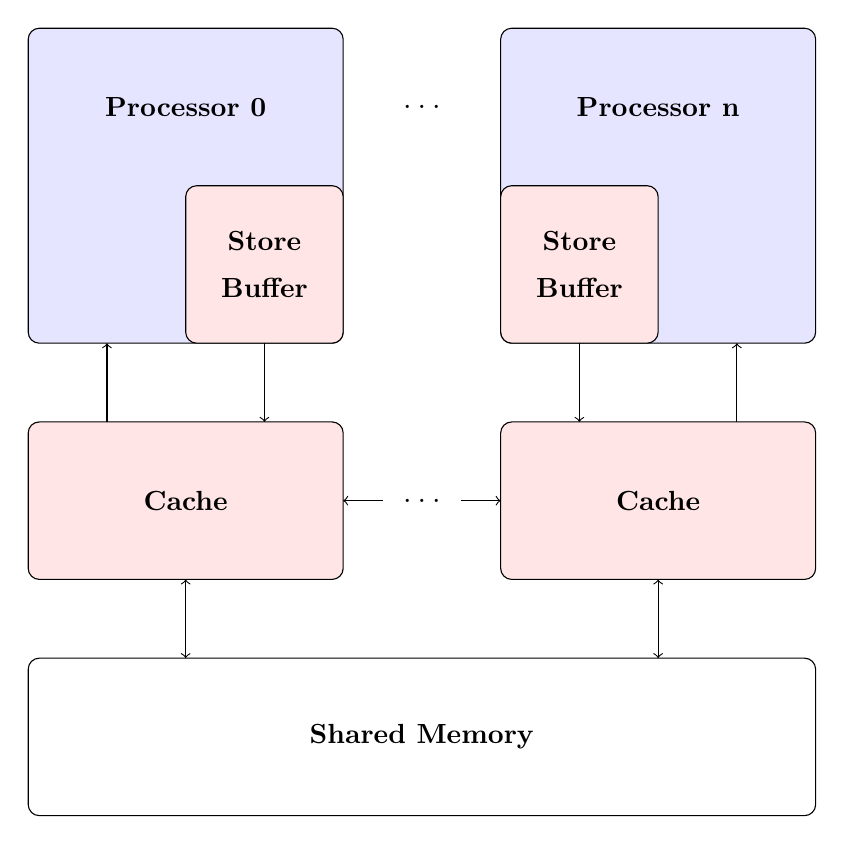
\begin{tikzpicture}

  % \draw[step=1cm,gray,very thin] (-5, 0) grid (5, -10);

  % processors
  \path [processor] (-5, 0) rectangle (-1, -4);
  \path (-3, -1) node (p-0) [] {\textbf{Processor 0}};

  \path [processor] (1, 0) rectangle (5, -4);
  \path (3, -1) node (p-n) [] {\textbf{Processor n}};

  % store buffers
  \path [buffer] (-3, -2) rectangle (-1, -4);
  \path (-2, -2.7) node (s-0) [] {\textbf{Store}};
  \path (-2, -3.3) node (b-0) [] {\textbf{Buffer}};

  \path [buffer] (1, -2) rectangle (3, -4);
  \path (2, -2.7) node (s-n) [] {\textbf{Store}};
  \path (2, -3.3) node (b-n) [] {\textbf{Buffer}};

  % caches
  \path [buffer] (-5, -5) rectangle (-1, -7);
  \path (-3, -6) node (c-0) [] {\textbf{Cache}};

  \path [buffer] (1, -5) rectangle (5, -7);
  \path (3, -6) node (c-n) [] {\textbf{Cache}};

  % heap
  \path [box] (-5, -8) rectangle (5, -10);
  \path (0, -9) node (heap) [] {\textbf{Shared Memory}};

  % arrows
  \path [draw, <-] (-4, -4) -- (-4, -5);
  \path [draw, ->] (-2, -4) -- (-2, -5);
  \path [draw, <->] (-3, -7) -- (-3, -8);

  \path [draw, <-] (4, -4) -- (4, -5);
  \path [draw, ->] (2, -4) -- (2, -5);
  \path [draw, <->] (3, -7) -- (3, -8);

  % \path [draw, <->] (-1, -6) -- (1, -6);
  \path [draw, <-] (-1, -6) -- (-0.5, -6);
  \path (0, -6) node (dots) [] {\large $\ldots$};
  \path [draw, ->] (0.5, -6) -- (1, -6);

  % dots
  \path (0, -1) node (dots) [] {\large $\ldots$};

\end{tikzpicture}

  \caption{System Architecture with Store Buffers}
  \label{fig:intro:store-buffer}
\end{figure}

When a variable is stored, then the new value is placed in the processor's store buffer, which can proceed immediately without having to wait for the store to do something about all the old values of that variable residing in other processors' caches.
% Each store buffer is allowed to voluntarily flush its contents back to memory, or may be forced to do so by certain instructions (memory barriers).
% store forwarding
In order to guarantee that each processor at least sees its own operation in program order, it first examines the store buffer before consulting the cache when loading a variable in a process called \emph{store forwarding}.
% flushes and memory barrier operations (explicit and implicit - OS issue a memory barrier before switching contexts)

\newpage

\begin{lstlisting}[style=c++, numbers=left, numberstyle=\footnotesize, numberblanklines=false, caption={Store Buffer Litmus Test}, label={fig:intro:code}]
#include <pthread.h>
#include <assert.h>

#define ACCESS(x) (*(volatile typeof(x) *) &(x))
#define READ(x) ({typeof(x) TMP = ACCESS(x); TMP;})
#define WRITE(x,v) ({ACCESS(x) = (v);})

static int w0 = 0;
static int w1 = 0;

static int r0 = 0;
static int r1 = 0;

static void * P0 (void * p)
{
  WRITE(w0, 1);
  r0 = READ(w1);
  return p;
}

static void * P1 (void * p)
{
  WRITE(w1, 1);
  r1 = READ(w0);
  return p;
}

int main ()
{
  pthread_t t[2];
  pthread_create (t + 0, 0, P0, 0);
  pthread_create (t + 1, 0, P1, 0);
  pthread_join (t[0], 0);
  pthread_join (t[1], 0);
  assert(r0 + r1);
  return 0;
}
\end{lstlisting}

\begin{figure}[!h]
  \centering
  \input{figures/c-trace.tex}
  \caption{Store Buffer Litmus Test Trace}
\end{figure}

\todo[inline]{x86 permits $\texttt{r0 = 0} \land \texttt{r1 = 0}$}

\todo[inline]{\texttt{experiments/demo/run.sh}: 177169 out of 1000000 failed = $\sim 17.7$ \% ($\sim 12$ min)}
\todo[inline]{only 82 out of 1000000 returned the perfectly legal outcome of 2}

\todo[inline]{lack of concrete, formal specifications what programmers can rely on}

\subsection{Toolchain}

\begin{figure}[h]
  \centering
  % styles
\tikzstyle{module} = [draw, fill=blue!10, text centered, rounded corners, minimum height=1cm, minimum width=2.5cm]
\tikzstyle{file} = [module, fill=red!10]

\begin{tikzpicture}[auto]

  \node [file] (program) {program};

  \node [module] (simulate) [above right=0cm and 1cm of program] {\texttt{simulate}};
  \path [draw, ->] (program.east) -- ++(0.5, 0) |- (simulate);

  \node [module] (solve) [below right=0cm and 1cm of program] {\texttt{solve}};
  \path [draw, ->] (program.east) -- ++(0.5, 0) |- (solve);

  \node [file] (trace) [below right=0cm and 1cm of simulate] {trace};
  \path [draw, ->] (simulate.east) -- ++(0.5, 0) |- (trace);
  \path [draw, ->] (solve.east) -- ++(0.5, 0) |- (trace);

  \node [module, dashed] (replay) [right= of trace] {\texttt{replay}} edge [<-, dashed] (trace);
  \path [draw, dashed, ->] (replay) -- (replay.north |- simulate) -| (trace.north);

\end{tikzpicture}

  \caption{Toolchain}
\end{figure}

\todo[inline]{components structured according to the mode they are used}
